\documentclass[a4paper]{article} %format de la feuille + type de document https://en.wikibooks.org/wiki/LaTeX/Document_Structure#Document_classes
%packages nécessaire pour nos besoins
\usepackage[utf8]{inputenc}
\usepackage[T1]{fontenc}
\usepackage[english,french]{babel}
\usepackage{amsmath}
\usepackage{amssymb,amsfonts,textcomp}
\usepackage{color}
\usepackage[dvipsnames]{xcolor}
\usepackage{array}
\usepackage{supertabular}
\usepackage{hhline}
\usepackage{hyperref}
\usepackage{capt-of}
\usepackage[pdftex]{graphicx}
\usepackage{sectsty}
\usepackage[most]{tcolorbox}
\usepackage{textcomp}
\usepackage{courier}
\usepackage[font={small,it}]{caption}
\usepackage{float}
\usepackage{graphicx}
\usepackage{subcaption}
\usepackage{caption}
\usepackage{multicol}
\usepackage{tikz}
\usepackage{makecell}

\usepackage[top=15mm,bottom=20mm,right=40mm,left=40mm]{geometry}
 
\usetikzlibrary {positioning,arrows,automata}


%Définition des couleurs
\definecolor{havelockBlue}{rgb}{0.004, 0.42, 0.73}
\definecolor{Monokaimagenta}{rgb}{0.86,0.08,0.24}

%utilisation de la couleur définie avant
%toutes les sections auront cette couleur
\sectionfont{\color{havelockBlue}}
\subsectionfont{\color{havelockBlue}}

\newcommand{\red}[1]{\textbf{\textcolor{OrangeRed}{#1}}}

%début du document
\begin{document}

%début d'un titre
\begin{titlepage}
            %centre les éléments
	\centering
	
	{\scshape\LARGE \color{Monokaimagenta} Laboratoire \\ Universal Asynchronous Receiver Transmitter \par}
	
	%espace vertical de 1 mms
	\vspace{1cm}
	
	{\Large\itshape Yohann Meyer \& Joel Schär\par}
	
	%http://www.personal.ceu.hu/tex/spacebox.htm
	\vfill
	Professeur\par
	%met le texte en gras 
	\textbf{Carlos Andrés Pena} \par% ajoute une ligne 
	\vspace{1cm}
	Assistant\par
	\textbf{Gaëtan Matthey}
	
	\vfill

            %affiche la date actuelle
	{\large \today\par}
	
%fin de la page de titre
\end{titlepage}

%démarre un chapitre, les nombres se mettent automatiquement et seront incrémenté quand un autre \section est rencontré
%voir https://en.wikibooks.org/wiki/LaTeX/Document_Structure#Sectioning_commands
\section{Description générale}
On appelle « trame » une suite de bits envoyés en série. Cette trame comprend dans l’ordre :
\begin{itemize}
\item Le « start-bit » toujours égal à 0.
\item Les bits de donnée (sur n bits) à transmettre.
\item Le bit de parité facultatif (non demandé dans ce labo).
\item Le bit de stop égal à 1.
\end{itemize}
De plus, l’état de repos de la ligne est fixé à 1.
\\ 
\begin{figure}[H]
    \centering
    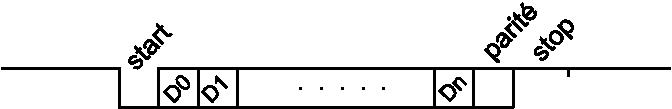
\includegraphics[width=.8\textwidth]{src/uart_1.jpg}
    \captionof{figure}{trame}
    \label{fig:trame}
\end{figure}


%saut à la ligne


%début d'un encadré avec la couleur définie plus haut
\begin{tcolorbox}[colframe=Monokaimagenta,colback=white]
\paragraph %démarre un paragraphe
{Spécification - Max 1/2 page } 
Nous avons réalisé la partie émetteur de l'UART. Notre circuit procède à l'envoi de 8 bits successifs donnés en entrée selon la forme demandée. Le circuit envoie la valeurs zéro sur deux temps d'horloge pour indiqué le début de l'envoi au circuit récepteur. L'envoi de chaque bits ce fait ensuite sur une durée de 4 temps d'horloge. Sur le quatrième temps l'instruction "Shift-right" est transmise au shift-register de manière a envoyer le bits suivant durant la séquence d'envoi suivante. A chaque shift on incrémente un compteur jusqu'a 7, qui nous indique la fin de la transmission et le retour à l'état d'attente.
%fin de l'encadré
\end{tcolorbox}

\section{Architecture}\

\begin{tcolorbox}[colframe=Monokaimagenta,colback=white]
\paragraph{Architecture - Max 1/2 page} 
\begin{figure}[H]
	\centering
	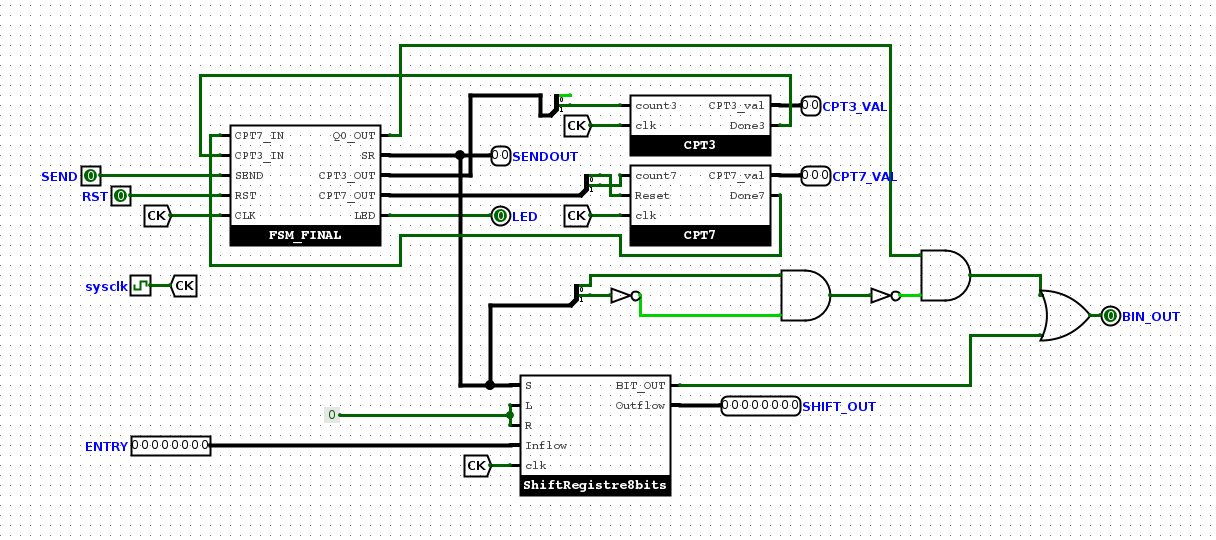
\includegraphics[width=\textwidth]{src/schema_UART}
	\captionof{figure}{UART}
	\label{fig:UART}
\end{figure}


\end{tcolorbox}


\section {Réalisation}
\subsection{Le bloc shift-register}
Ce bloc sur 8 bits a 4 modes de fonctionnement. Vous devez le refaire entièrement avec des bascules et des multiplexeurs.

\begin{tcolorbox}[colframe=Monokaimagenta,colback=white, breakable, enhanced]
\paragraph{Conception et tests - Max 1 page}
Insérez une capture d’écran pour présenter votre bloc shift-register. Expliquez brièvement son fonctionnement.
Indiquez comment vous avez testé les 4 modes de fonctionnement afin de le valider.
Remplacez le texte ci-dessus par vos réponses (à l’intérieur du cadre rouge)\\

\begin{figure}[H]
	\centering
	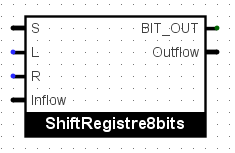
\includegraphics[scale=0.5]{src/SR_8b_bloc}
	\captionof{figure}{Bloc du Shift Register 8 bits}
	\label{fig:SR_8b_bloc}
\end{figure}
Nous avons pour le bloc Shift Register 8 bits les entrées, sorties suivantes : 
\begin{itemize}
	\item Le signal de commande "S" qui donne les instructions sur le mode de fonctionnement du registre.
	\item Les entrées "L" et "R" qui permette d'entrer une valeur depuis la gauche ou la droite au moment du shift. 
	Dans ce laboratoire, nous utilisons le comportement de base de chargement et fixons donc ces valeurs à 0.
	\item Un bus "Inflow" qui permet d'entrer la séquence a charger.
	\item Un bus "Outflow" qui prend les valeurs des huit état du registre, utile pour avoir une meilleure vision de la situation (debugging).
	\item Le bit de sortie qui prend la valeur du bit de poids faible en sortie du registre.
\end{itemize}

Le signal de commande est codés comme suit :
\begin{center}
	\begin{tabular}{c|l}
		00	&	Hold\\
		01	&	Load\\
		10	&	Shift Right\\
		11	&	Shift Left\\
	\end{tabular}
\end{center}

Le shift register 8 bits que nous avons conçu est une combinaison de deux shift Register 4 bits interconnectés. 
\begin{figure}[H]
	\centering
	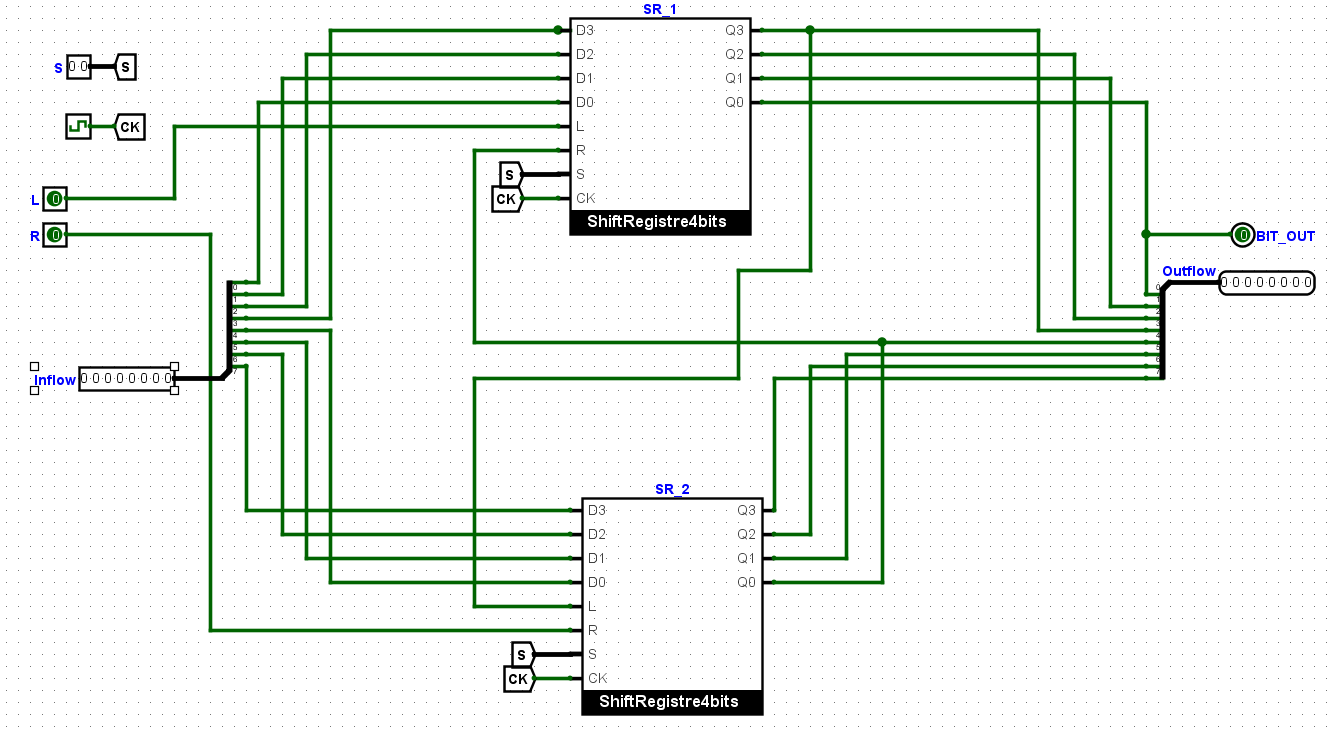
\includegraphics[width=\textwidth]{src/SR_8b}
	\captionof{figure}{Shift Register 8 bits}
	\label{fig:SR_8b}
\end{figure}
Le registre "SR\_2" a 4bits prend en entrée les bits de poids fort (gauche) du flux d'entrée. Il transmet sont bit de poids faible Q0 au second registre "SR\_1" qui traite les bits de poids faible. La flux "ouflow" de sortie est la combinaison des sortie "Q0-Q3" des deux blocs et le "bit-out" le bit de poids faible de cette séquence.

Chaque "shift register" à 4bits et structuré comme suit.
\begin{figure}[H]
	\centering
	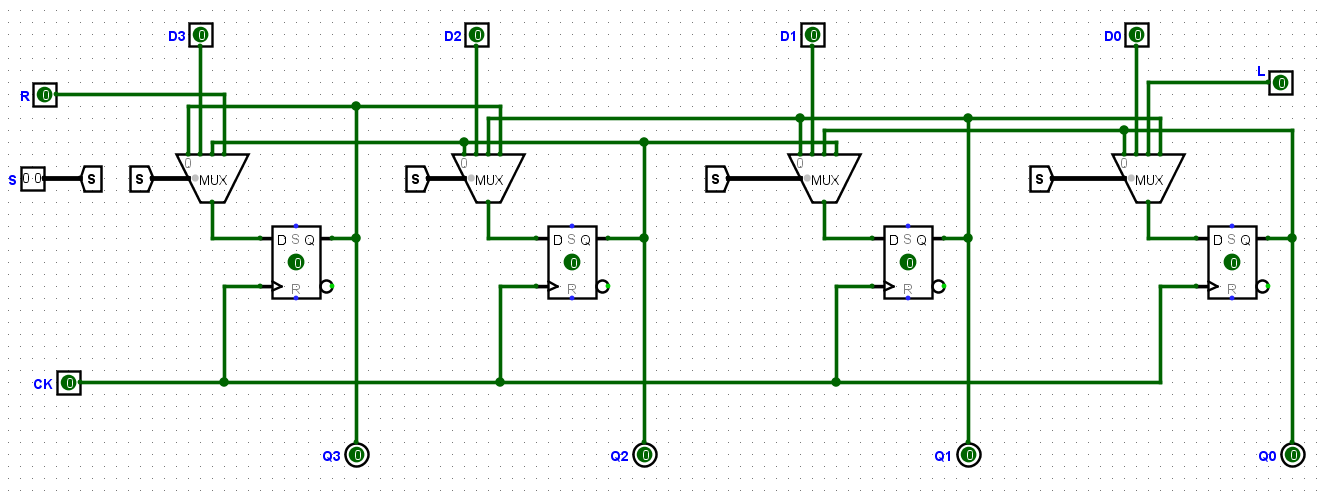
\includegraphics[width=\textwidth]{src/SR_4b}
	\captionof{figure}{Shift Register 4 bits}
	\label{fig:SR_4b}
\end{figure}
Chaque bascule prend en entrée la valeur donnée par un multiplexer en fonction du code de commande. Cette valeur est la valeur du bit donné par le flux d'entrée ("inflow" : Shift Register 8bits) au moment de la commande "Load" (01). La valeur de l'état "Q+1" lors d'un "Shift Left" (10). La valeur de l'état "Q-1" lors d'un "Shift Right" (11). La valeur "Q" actuelle en mode "Hold" (00). Le changement se fait à chaque flanc montant de l'horloge.
\end{tcolorbox}

\subsection{Le bloc compteur 0-3}
Le premier compteur demandé compte de 0 à 3. Ce compteur comprend une entrée de remise à 0 synchrone et une sortie indiquant que le compteur a atteint sa valeur maximum.
	
\begin{tcolorbox}[colframe=Monokaimagenta,colback=white, breakable, enhanced]
\paragraph{Conception et tests - Max 1 page }
Insérez une capture d’écran pour présenter votre bloc compteur 0-3. Expliquez sa réalisation et son fonctionnement.
Indiquez comment vous avez testé les différents modes de fonctionnement afin de le valider. Vous pouvez ajouter un chronogramme.
Remplacez le texte ci-dessus par vos réponses (à l’intérieur du cadre rouge)\\



Le compteur 0-3 que nous avons implémenté, reçoit comme entrées l'indication de compter, et transmet en sortie la valeur à laquelle il se trouve ainsi qu'un bit indiquant le compteur à terminé de compter jusqu'à 3.\\	
\begin{figure}[H]
	\centering
	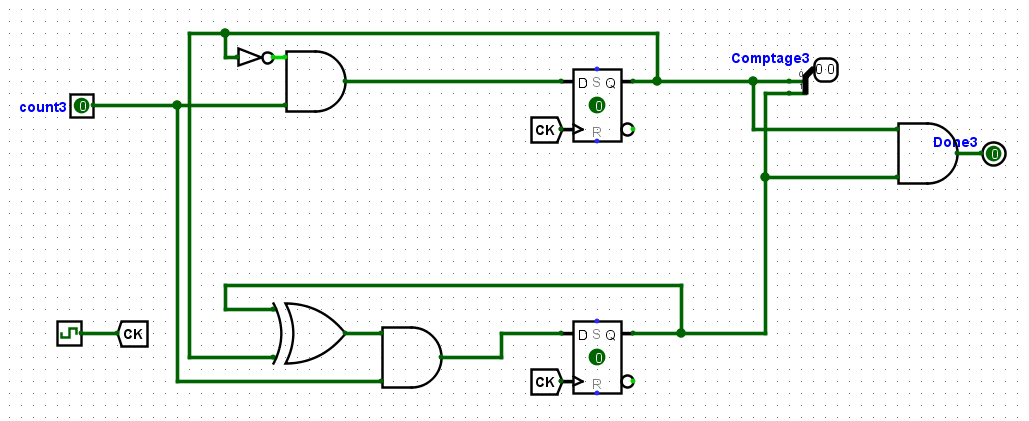
\includegraphics[width=\textwidth]{src/CPT_03_1}
	\captionof{figure}{Compteur de 0 à 3}
	\label{fig:CPT_03_1}
\end{figure}
Selon les besoins du laboratoire et pour des raison d'optimisation si la valeur d'entrée n'est pas à 1 et ne donne pas l'ordre de compter, le compteur se remet automatiquement à 0. Il est donc prêt à recommencer une séquence. Nous n'avons jamais besoin d'interrompre ce compteur et de garder sa valeur en mémoire. L'utilisation d'une commande de remise à zéro est donc superflue.\\

\begin{figure}[H]
	\centering
	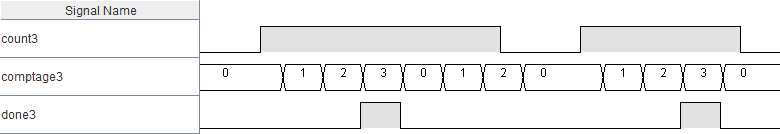
\includegraphics[width=\textwidth]{src/chrono_CPT3_1}
	\captionof{figure}{Chronogram Compteur de 0 à 3}
	\label{fig:chrono_CPT_03_1}
\end{figure}
Ce chronogram illustre le fonctionnement du compteur et met en évidence la remise à zéro automatique du compteur.


\begin{multicols}{2}
	\begin{tabular}{c|l l}
		$C,Q_1,Q_0$ & $Q_1^+$& $Q_0^+$ \\
		\hline
		100	&	0&1\\
		101	&	1&0\\
		110	&	1&1\\
		111	&	0&0\\
	\end{tabular}
	

	\begin{equation*}
	Q_1^+ = C(Q_0 + Q_1)
	\end{equation*}
		\begin{equation*}
			Q_0^+ = C\overline{Q_0}
		\end{equation*}

\end{multicols}
Pour des raisons de conception de notre machine d'état, la transition entre l'état dans lequel le compteur compte et le celui ou le shift de la valeur se fait, nécessite un battement d'horloge. De ce fait nous avons utilisé un compteur qui donne l'indication de fin de comptage a 2 et non 3, cela étant illustré par la porte not du and de sortie.
\begin{figure}[H]
	\centering
	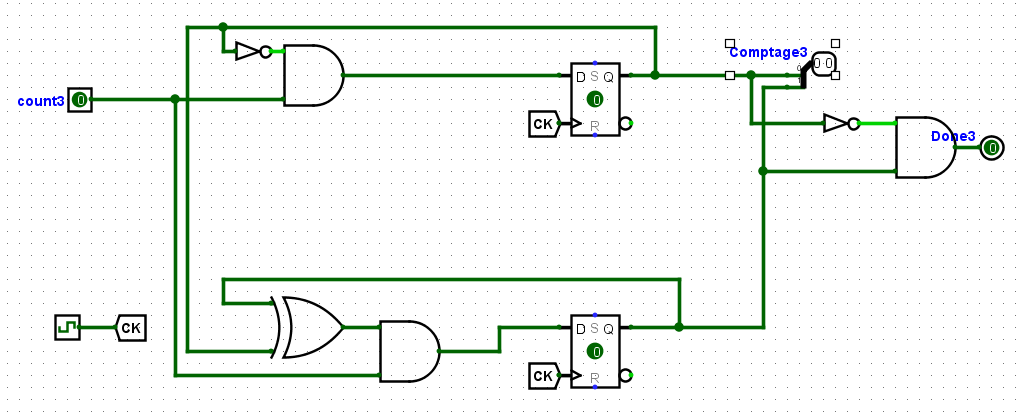
\includegraphics[width=\textwidth]{src/CPT_03_2}
	\captionof{figure}{Compteur de 0 à 2}
	\label{fig:CPT_03_2}
\end{figure}
\end{tcolorbox}

\subsection{Le bloc compteur 0-7}
Le deuxième compteur demandé compte de 0 à 7. Ce compteur comprend une entrée de remise à 0 synchrone, une entrée enable pour l’activer et une sortie indiquant que le compteur a atteint sa valeur maximum.

\begin{tcolorbox}[colframe=Monokaimagenta,colback=white, breakable, enhanced]
\paragraph{Conception et tests - Max 1 page}
Insérez une capture d’écran pour présenter votre bloc compteur 0-7. Expliquez sa réalisation et son fonctionnement. Inutile de reprendre les explications du paragraphe précédent 3.2. Expliquez simplement ce que vous avez dû changer ou rajouter pour passer du compteur 0-3 au compteur 0-7.
Indiquez comment vous avez testé les différents modes de fonctionnement afin de le valider. Vous pouvez ajouter un chronogramme.
Remplacez le texte ci-dessus par vos réponses (à l’intérieur du cadre rouge)\\

Le compteur 7 que nous avons implémenté nous permet de compter le nombre de bits qui on été envoyé, de manière à savoir quand la séquence de 8 bits à été envoyée au complet.\\
Ce compteur doit donc garder la valeur en mémoire quand l'ordre le bit "count" est a zéro et reprendre dans le cas contraire. Il est donc également nécessaire d'avoir une entrée "Reset" qui permet de le remettre à 0.\\
\begin{figure}[H]
	\centering
	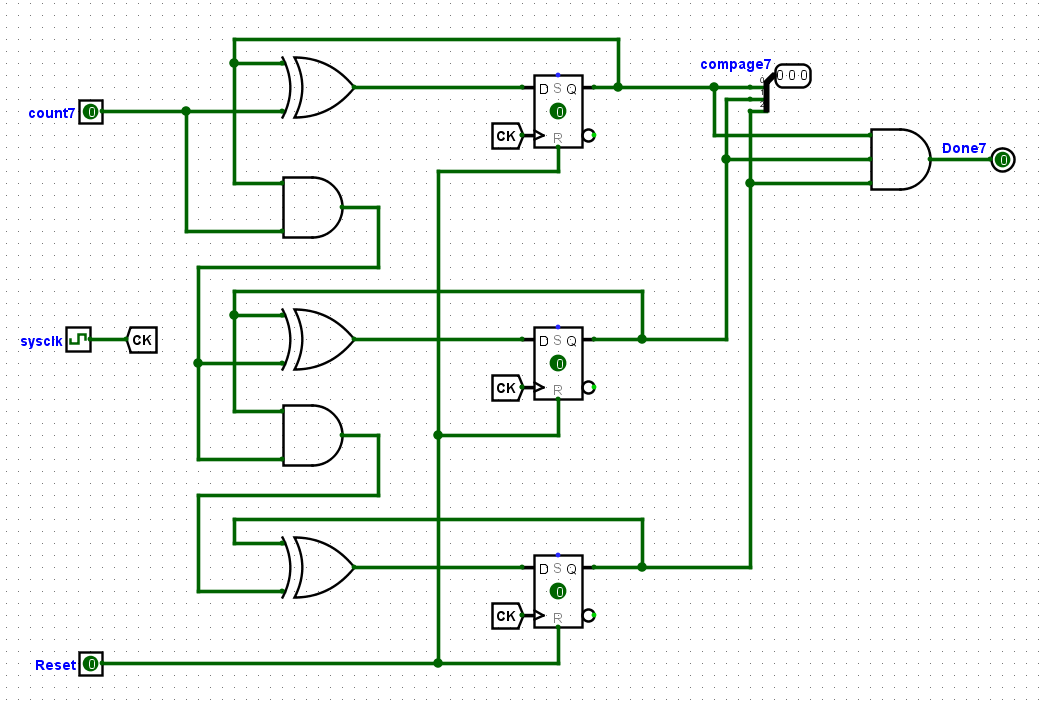
\includegraphics[width=\textwidth]{src/CPT_07}
	\captionof{figure}{Compteur de 0 à 7}
	\label{fig:CPT_07}
\end{figure}
	
Pour implémenter le compteur à 7 (3bits), on précède sur la base d'un compteur à 3 (2bits) et on rajoute une fois la séquence de portes logiques.\\
Depuis la table d'états suivante :
\begin{center}
	\begin{tabular}{c|c|c}
			& 	Send = 0 &	Send = 1\\ \hline 
		00	&	00		 & 01 \\
		01	&	01	     & 10 \\
		10	&	10       & 11 \\
		11	&	11 		 & 00 \\
		$Q_1Q_0$&$Q_1^+Q_0^+$&\\
	\end{tabular}
\end{center}
Depuis cette table on peut en sortie les équations suivante : 
\begin{align*}
 Q_0^+ &= \overline{S}Q_0 + S \overline{Q_0} = S \oplus Q_0 \\
 Q_1^+ &= \overline{S}Q_1+Q1\overline{Q0} + S\overline{Q1}Q0 =  Q1\overline{SQ0} + \overline{Q1}SQ0= Q_1 \oplus (SQ_0) 
\end{align*}
On peut donc établir le logigramme suivant:
\begin{figure}[H]
	\centering
	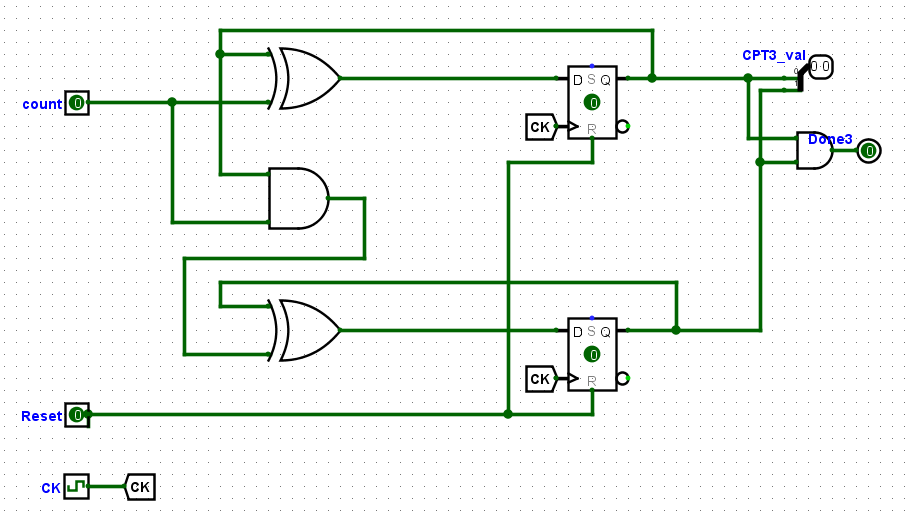
\includegraphics[width=\textwidth]{src/CPT_03}
	\captionof{figure}{Compteur de 0 à 3}
	\label{fig:CPT_03}
\end{figure}

Pour ensuite passer au compteur à 7 (3bits) on ajoute une fois la séquence de porte suivante :
\begin{figure}[H]
	\centering
	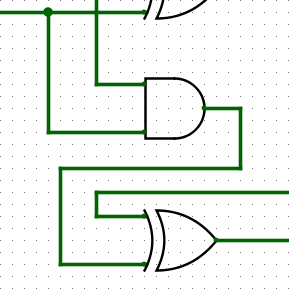
\includegraphics[scale=0.5]{src/sequence_CPT3}
	\captionof{figure}{Séquence de porte}
	\label{fig:sequence_CPT3}
\end{figure}

Ainsi qu'une bascule supplémentaire pour obtenir le résultat suivant.

\begin{figure}[H]
	\centering
	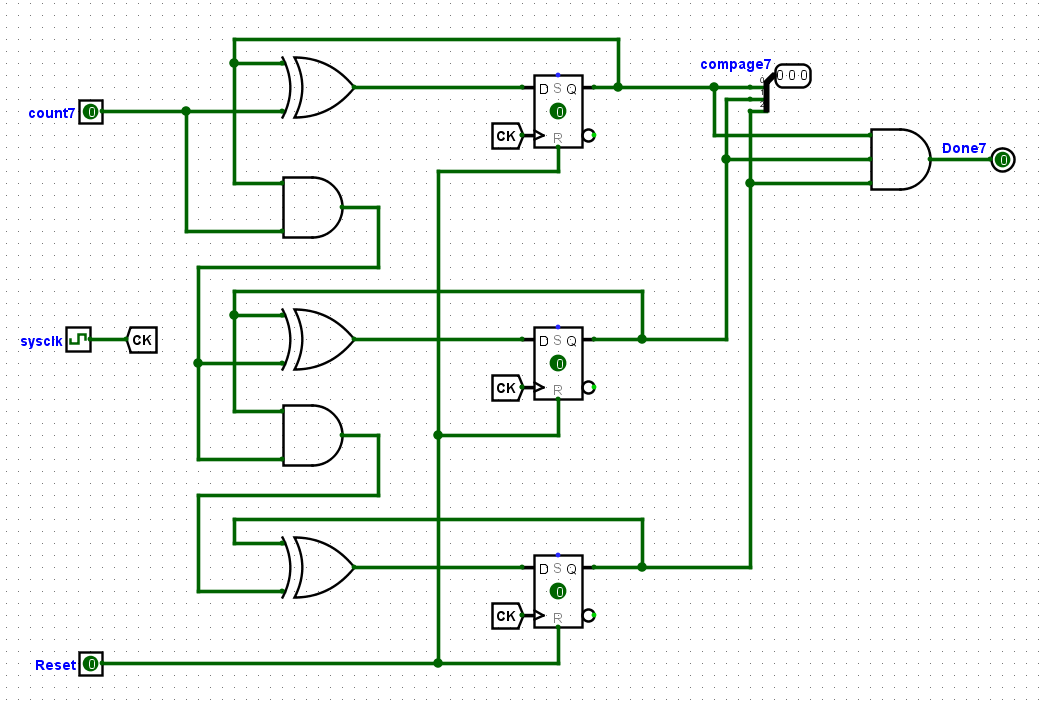
\includegraphics[width=\textwidth]{src/CPT_07}
	\captionof{figure}{Compteur de 0 à 7}
	\label{fig:CPT_07}
\end{figure}

Selon le chronogram établi sur la base de ce compteur on vérifie que le compteur fonctionne selon le cahier des charges.
\begin{figure}[H]
	\centering
	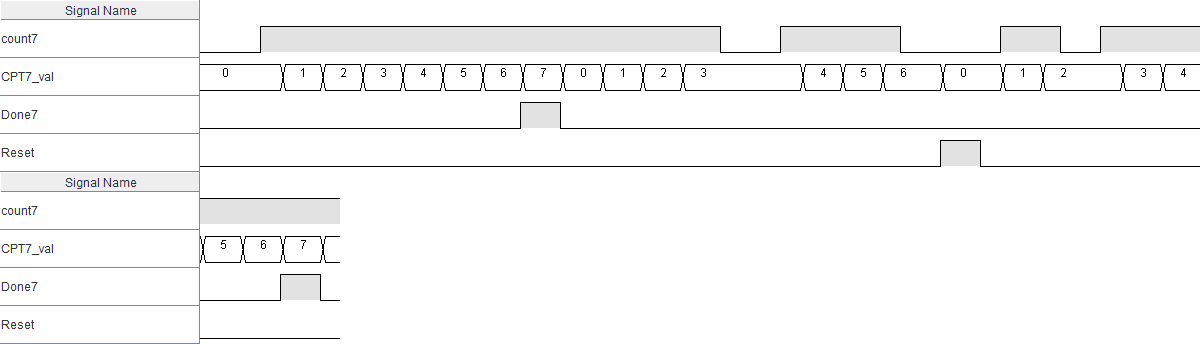
\includegraphics[width=\textwidth]{src/chrono_CPT7}
	\captionof{figure}{chronogram du compteur de 0 à 7}
	\label{fig:chronogramCPT7}
\end{figure}


\end{tcolorbox}

\subsection{La machine d’état}
Cette machine d’état de type 1 parmi M contrôle les deux compteurs et le shift register. 
\begin{tcolorbox}[colframe=Monokaimagenta,colback=white, breakable, enhanced]
\paragraph{Conception Max 3 pages}
Précisez les entrées et sorties de votre machine d’état
Insérez un graphe des états et une table des états. Donnez des explications sur le fonctionnement de votre machine. Quel est son Type ?
Donnez les équations des états futurs et insérez une capture d’écran de la réalisation de votre machine.
Remplacez le texte ci-dessus par vos réponses (à l’intérieur du cadre rouge)
\\

Nous avons conçu une machine d'état one-hot sur le principe d'une machine de Moore composée de 4 états. 
\begin{itemize}
	\item "Wait"\\
	La machine est en état d'attente jusqu'à ce que le signal "send" soit reçu.
	\item "Start"\\
	La machine lance la séquence d'envoi, et charge les valeurs d'entrées dans le registre.
	\item "Send"
	La machine compte 4 battements d'horloge.
	\item "Shift"
	La machine envoie le signal au registre pour faire un "shift right".
\end{itemize}

\begin{center}

\begin{tikzpicture}[->,>=stealth',shorten >=1pt,auto,node distance=2.8cm,
                    semithick]
  \tikzstyle{every state}=[fill=Monokaimagenta,draw=none,text=white]

\node[initial,state] (A) {\makecell[l]{$Wait$\\1000}};
\node[state] (B) [below right of = A] {\makecell[l]{$Load$\\0100}};
\node[state] (C) [below left of = B] {\makecell[l]{$Send$\\0010}};
\node[state] (D) [below left of = A] {\makecell[l]{$Shift$\\0001}}; 



\path (A) edge [loop above] node {$0XX$} (A);
\path (A) edge [bend left] 	node {$1XX$} (B);
 

\path (B) edge [bend left]	node {} (C);
\path (C) edge [loop below] node {$X00$} (C);
\path (D) edge [bend left]	node {$X1X$} (A);
\path (D) edge [bend left]	node {$X0X$} (C);
\path (C) edge [bend left]	node {$XX1$} (D);

    \end{tikzpicture} \\
    $Entrees$ \\ $SC_7C_3$ \\$ XXX$
\end{center}

Sur la base de ce graphe et vu que nous avons un codage one-hot, nous avons ressortis les équations des états future suivantes:\\
$[Wait]  Q_0^+ = Q_3C_7 + \bar{Q_3}\bar{Q_2}\bar{Q_1}\bar{S}$* \\
$[Load ] Q_1^+ = Q_0S $\\
$[Send]  Q_2^+ = Q_1 + Q_3\overline{C_7} + Q_2\bar{C_7}\bar{C_3}$\\
$[Shift] Q_3^+ = Q_2C_3$\\

*Ce deuxième groupe correspond à notre volonté d'être dans l'état 1000 ($Q_0$) au repos.

Les entrées sorties dont nous avons besoin pour la machines d'état se retrouvent dans le bloc de la machine.
\begin{figure}[H]
	\centering
	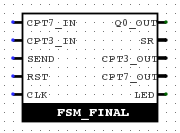
\includegraphics[scale = 0.8]{src/bloc_FSM}
	\captionof{figure}{Bloc de la machine d'états}
	\label{fig:bloc_FSM}
\end{figure}

\begin{itemize}
	\item Entrées :
	\begin{itemize}
		\item CPT3 : retour de la valeur de CPT3 indiquant le comptage à 3
		\item CPT7 : retour de la valeur de CPT7 indiquant le comptage à 8
		\item Send : indication du début d'un envoi (selon le bouton send)
		\item Reset: reset de la machine d'état vers sont état d'attente ("Wait")
		\item clk  : signal d'horloge
	\end{itemize}
	\item Sorties :
	\begin{itemize}
		\item Q$_0$\_out : valeur de l'état Q$_0$, indique quand la machine est en attente
		\item SR		 : code commande pour le registre a décalage
		\item CPT3\_OUT  	 : bit de commande pour lancer le comptage de CPT3
		\item CPT7\_OUT	 : bit de commande pour lancer le comptage de CPT7
		\item LED        : signal pour la LED, indique quand une séquence d'envoi est terminée
	\end{itemize}
\end{itemize}

Sur cette base nous avons implémenté la machine d'état suivante.
\begin{figure}[H]
	\centering
	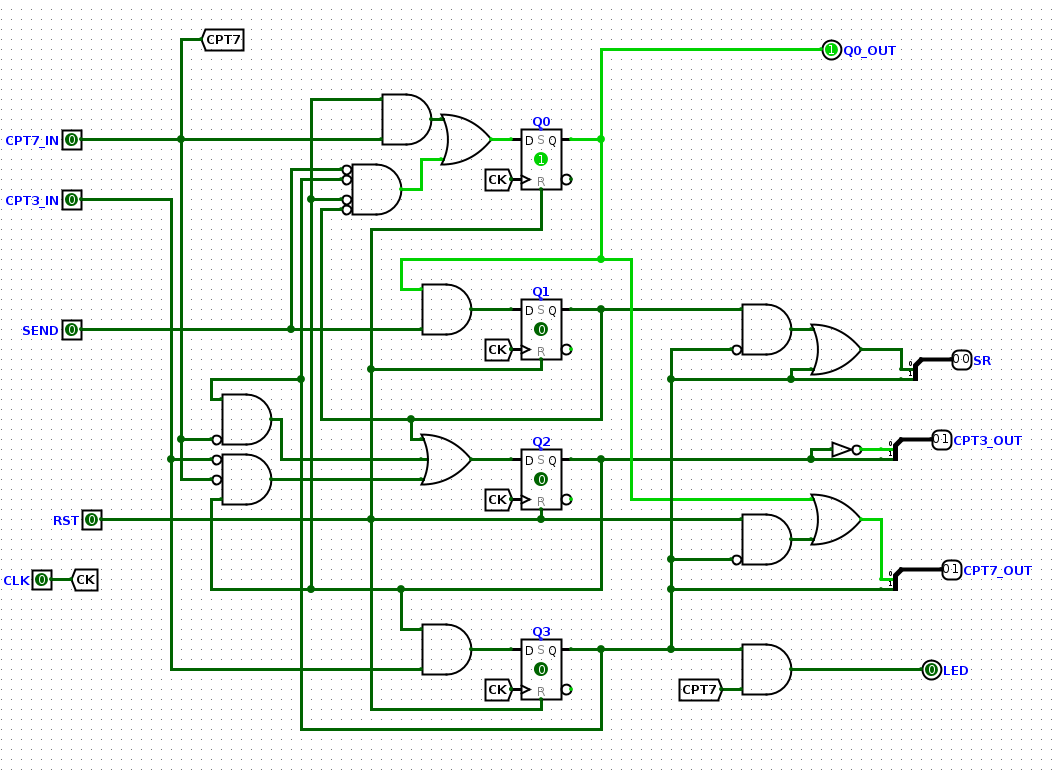
\includegraphics[width=\textwidth]{src/FSM}
	\captionof{figure}{Logigram de la machine d'état}
	\label{fig:FSM}
\end{figure}

\red{ajouter les détails sur le fonctionnement}\\
séquence de la machine et action des états :
\begin{enumerate}
	\item wait (aucune action)\\
	(entrée : send) \textrightarrow\ start
	\item start (signal au SR "Load", bin\_out à 0, 2 coup d'horloge)
	\item send (signal a CPT3\_C "count")\\
	(entrée : CPT3) \textrightarrow\ shift
	\item shift (signal au SR : "shift", CPT7 count) (1 coup d'horloge)\\
	\textrightarrow\ send
	\item send \\
	$ \quad \vdots \quad \vdots$
	\item shift (signal au SR : "shift", CPT7 count) (1 coup d'horloge)\\
	(entrée : CPT7) \textrightarrow\ wait
\end{enumerate}
\begin{tabular}{|c c c c|}
\hline
Entrées & Etat & Sortie  (SR,C3,C7) & Commentaire\\
\hline
Send = 0 & Wait & 00 0 0 & 1 tick\\
Send = 1 & Load & 01 0 0 & 1 tick\\
CPT3,7 = 0 & Send & 00 1 0 & compte a 3\\
CPT3 = 1 CPT7 = 0& Shift & 11 0 1 & 1 tick\\
CPT7 = 1 & Wait & 00 0 0 & compte a 8\\
\hline
\end{tabular}

\end{tcolorbox}
\section {Intégration et simulation}
\subsection{Intégration}
Suivant votre partie à concevoir, vous devez réalisé l’UART en interconnectant les différents blocs. 
\begin{tcolorbox}[colframe=Monokaimagenta,colback=white, breakable, enhanced]
\paragraph{Réalisation et simulation Logisim - Max 1 page}
Insérez une capture d’écran de l’UART complet sous Logisim
Expliquez le fonctionnement global de l’UART
Remplacez le texte ci-dessus par vos réponses (à l’intérieur du cadre rouge)
\\

Avec tous les éléments implémentés précédemment nous les avons combiné de manière à obtenir une UART sous la forme d'un émetteur 8 bits.
\begin{figure}[H]
	\centering
	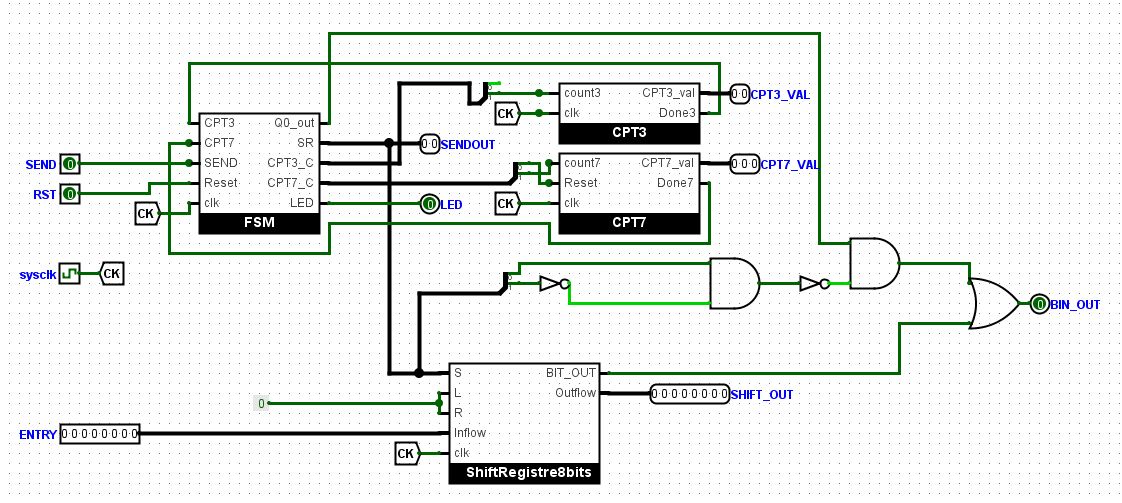
\includegraphics[width=\textwidth]{src/UART}
	\captionof{figure}{UART, émetteur}
	\label{fig:UART4}
\end{figure}

\begin{itemize}
	\item le signal "reset" permet de remettre tout l'unité dans son mode d'attente prête à envoyer une séquence.
	\item le signal "send" transmet à la machine d'état de sortir du mode d'attente et de commencer à envoyer la séquence. Quand il est à zéro, on reste dans l'état d'attente $Q_0$. Il n'est pas nécessaire d'avoir le signal a 1 tout au long de l'envoi, mais cela ne changerait rien dans le cas.
	\item l'envoi se fait par la sortie Bin\_out selon l'avancement de a machine d'état et les valeurs entrées dans le bus "entry". La construction de portes logiques utilisant Q0\_out permet d'avoir un état au repos = 1 et égal à 0 pendant deux coups d'horloges pour signifier le début du chargement.
	\item une fois la séquence terminée la machine d'état envoie le signal de fin par la sortie "LED" et repasse en mode d'attente.
	\item le signal sur Bin\_out est alors à 1 selon la combinaison du signal "SR" de la machine d'état et de la valeur Q$_0$\_out qui est à 1. La figure suivante montre que l'on obtient 0 pendant le Load et 1 le reste du temps.
\end{itemize}
\begin{figure}[H]
	\centering
	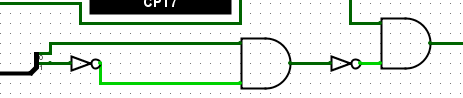
\includegraphics[scale=0.5]{src/bin_out_1}
	\captionof{figure}{système logique bin\_out}
	\label{fig:bin_out_1}
\end{figure}




\end{tcolorbox}
 \subsection{Simulation sous Logisim}
L’UART réalisé est ensuite testé en simulation sous Logisim.
\begin{tcolorbox}[colframe=Monokaimagenta,colback=white, breakable, enhanced]
\paragraph{Réalisation et simulation Logisim - Max 2 pages}
Indiquez comment vous simulez votre UART sous Logisim (seul ou avec le générateur fourni), ET avec un UART d’un autre groupe (indiquez quel groupe)
Insérez un ou plusieurs chronogrammes, annotez-le(s) et expliquez pourquoi le fonctionnement est correct et conforme aux spécifications.
Remplacez le texte ci-dessus par vos réponses (à l’intérieur du cadre rouge)
\\
\end{tcolorbox}
 \subsection{Synthèse et test de fonctionnement réel}
Synthèse et configuration du matériel, test de fonctionnement.
L’UART finalement synthétisé et chargé dans une carte, une carte émetteur sera reliée à une carte récepteur afin de tester une transmission de données.
\begin{tcolorbox}[colframe=Monokaimagenta,colback=white, breakable, enhanced]
\paragraph{Essais avec une carte - Max 1 page}
Indiquez comment vous faites le test (et avec un groupe différent de la simulation). Quelles données choisissez-vous pour faire les essais ?Vous devez faire valider votre circuit en fonctionnement au professeur ou à l’assistant
Commentez brièvement votre expérience dans cette étape en mentionnant, par exemple, des éventuelles difficultés à faire fonctionner le circuit ou à configurer la carte, etc.
Remplacez le texte ci-dessus par vos réponses (à l’intérieur du cadre rouge) \\
Au moment des tests, notre émetteur étant encore légèrement buggé, il a été impossible de procéder à des tests constructifs. Après de mineurs ajustements (clock sur 4 temps et non pas 5 et ajout de la valeur 1 pour la sortie au repos), un test a été réalisé avec le récepteur de l'assistant. \\
On a pu constater le succès de la transmission de plusieurs valeurs de suite (192 et 193 entre autres), démontrant
le fonctionnement correct des différentes fonctionnalités (reset, send,..). \\
On a profité des différentes led en dessus des boutons de valeurs pour afficher les valeurs de nos compteurs, permettant une vérification plus clair du bon déroulement de l'expérience (n'en ayant pas besoin autrement sur l'émetteur).
L'entiereté de la partie chargement sur carte n'a pas posé problème, ayant déjà pratiqué cela dans un précédent laboratoire. 
\begin{figure}[H]
	\centering
	\includegraphics[scale=0.2]{src/FPGA.jpg}
	\captionof{figure}{logiciel sur carte en transmission}
	\label{fig:FPGA}
\end{figure}
\end{tcolorbox}
\section {Conclusion}
\begin{tcolorbox}[colframe=Monokaimagenta,colback=white, breakable, enhanced]
\paragraph{Conclusion - Max 1/2 page}
Cette section est libre pour que vous fassiez une analyse critique de votre laboratoire
Commentez et analysez 
les résultats, 
les difficultés et les succès
Rédigez quelques conclusions personnelles
Donnez vos impressions et analysez votre expérience dans ce laboratoire
Discutez de ce que vous avez appris (ou pas)
Analysez votre travail, votre implication
Evitez les banalités et les lieux communs
ETCAETERA…
\\
On retrouve dans ce laboratoire une excellente mise en pratique des systèmes séquentiels. \\
La difficulté principale (pour nous) s'est posée dans la modélisation du problème par un graphe d'état. La première itération utilisait 5 états différents, mais on s'est rapidement rendu compte que 4 états suffisaient. \\
Cela fait, le codage en lui-même sur logisim n'était presque qu'une formalité, nos équations étant particulièrement valable (le seul rajout qui a été fait par après fut le groupe qui nous met dans l'état $Q_0$ en attente, au lieu de rester dans un état 0000 inexistant). \\
Il est très gratifiant de passer d'une conception de l'esprit à une machine entièrement fonctionnel permettant de communiquer avec une autre en sachant précisement comment tout fonctionne, des portes logiques aux bascules bistables. \\
Ce laboratoire nous a permis de nous rendre compte de comment créer une notion de temporalité dans des systèmes combinatoires et en faire des systèmes séquentiels. \\

\end{tcolorbox}


\end{document}